\documentclass{article}

\usepackage{fullpage}
\usepackage{titlesec}
\usepackage{parskip}
\usepackage{graphicx}
\usepackage{bold-extra}
\usepackage{caption}
\usepackage{subcaption}

%\titleformat{\section}{\normalsize\bf}{\thesection \hspace{5pt}}{0em}{}
%\titleformat{\subsection}{\normalsize\bf}{\thesubsection \hspace{5pt}}{0em}{}

\begin{document}

\centerline{\Large{\textbf{Distributed Multi-Heuristic A* (HAMSTAR)}}}
\centerline{Noam Brown, Aram Ebtekar, Yuzuko Nakamura}
\centerline{15-712 Fall 2014 Final Project Report}

\section{Abstract}

A* is a popular graph search algorithm used in many artificial intelligence applications. The original A* algorithm makes use of a single heuristic to prioritize exploration through a graph, but a variation on the algorithm known as multi-heuristic A* (MHA*) makes use of multiple heuristics to more quickly arrive at approximate solutions. For this project we implemented a distributed version of MHA*, with one process per heuristic. We show... [performance]
%TODO: Highlight important results

\section{Introduction}

Weighted A* is a simple, heuristic-based search algorithm used in artificial intelligence applications such as robotics and games. A heuristic function estimates the remaining distance from any state to the goal. Whereas a breadth-first method such as Dijkstra's algorithm will expand exponentially many states relative to the goal distance, wA* will focus toward the goal when guided by a good heuristic. If the heuristic is \textbf{admissible}, meaning it never overestimates the true distance, then the solution is guaranteed to be optimal to within the weight factor. If it meets a stronger condition called \textbf{monotonicity}, then no state needs to be expanded more than once.

Finding good efficiently computable heuristic functions is difficult and, moreover, finding an admissible heuristic function that is reasonably accurate over the entirety of the search space is often not practical. Multi-heuristic A* (MHA*) \cite{Aine14} is an alteration of the A* algorithm that allows multiple arbitrary heuristics to guide the search; to retain the optimality bound, it is only necessary to use one monotone heuristic, called an ``anchor". Where the shortcomings of each individual heuristic may result in local optima which trap the search, the ability to change heuristics can provide an escape.

In their work, Aine et al. propose MHA* in two flavors: Independent Multi-Heuristic A* (IMHA*), where path cost and shortest path information are tracked separately for each heuristic, and Shared Multi-Heuristic A* (SMHA*), where shared knowledge of path cost and shortest path information are shared and updated by all heuristics. IMHA* would be almost trivial to parallelize, as it requires minimal communication between the searches run by different heuristics. SMHA* uses a very large amount of frequently updated shared memory, presenting major challenges for parallel settings, let alone distributed systems settings.

Nonetheless, as SMHA* is the more effective of the two (enabling more co-operation and less redundancy between heuristics), we decided for our project to implement a distributed version of SMHA*.

\section{Relevant Work}

Our work is directly based on Aine et al.'s original multi-heuristic A* search \cite{Aine14} mentioned above. There exists past work on the paralellization of A*; in particular, Phillips et al. \cite{phillips2014pa} were able to achieve parallelization while retaining wA*'s guarantee of suboptimality without reexpansions. This method of parallelization makes inferences on when it is safe to expand multiple nodes in parallel, by resolving dependencies between potential optimal paths. Their speed gains are dependent on the expansion operation being expensive enough to dominate the cost of computing these dependency checks, which may not be the case for all problems. By contrast, our method parallelizes the search process by simultaneously expanding nodes chosen by different heuristics, instead of multiple nodes chosen by a single heuristic. We allow each state to be expanded by each heuristic at most once and, furthermore, no state will be expanded by a non-anchor heuristic which has received a message from another heuristic after the latter has expanded the same state. In other words, aside from communication latency, no state will be expanded more than twice.

\section{System Description}

\begin{figure}
\centering 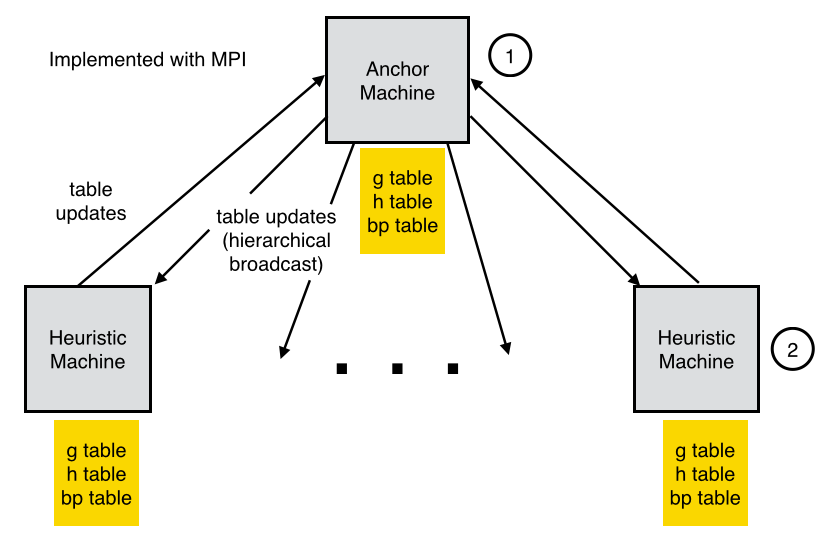
\includegraphics[width=5.0in]{system-diagram}
\caption{A diagram of our system. One machine starts up the others and runs the admissible anchor search. The other machines run their individual heuristics. Communication is done using MPI. 
\textcircled{1}\textbf{Anchor:} Starts heuristic machines; performs state expansions using anchor heuristic; receives, resolves, and broadcasts table updates; checks for termination conditions. \textcircled{2}\textbf{Heuristic:} Expands a likely state (chosen using heuristic); updates path cost to its successors; communicates updates to anchor; checks for termination conditions}
\label{fig:sysdiag}
\end{figure}

An overview of our system is in Figure \ref{fig:sysdiag}. The main (anchor) machine starts up other heuristic machines. Each machine runs its own heuristic, with the anchor machine's being the admissible heuristic. Each of the non-anchor heuristic machines periodically sends updates of the data structures (tables containing shortest path information found so far) to the anchor machine, which compares the data it receives and sends out table updates of the best paths known so far to all other nodes.

\begin{figure}
\centering 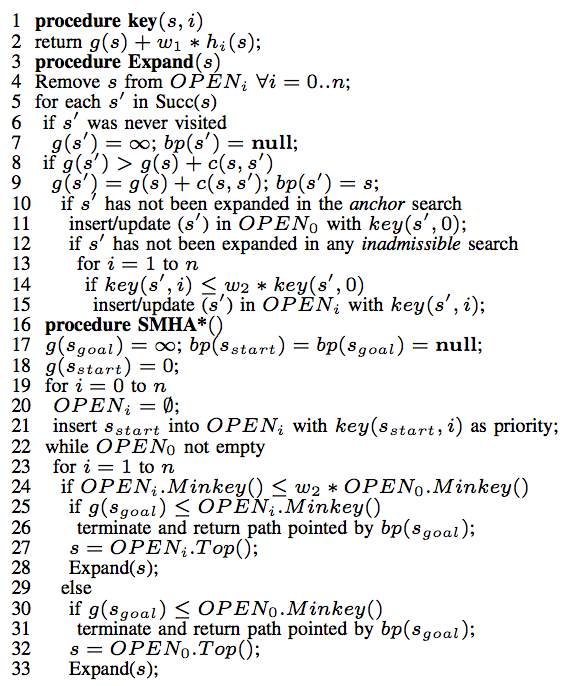
\includegraphics[width=3in]{pseudocode}
\caption{Pseudocode from Aine et al., detailing the original single-threaded version of the algorithm we parallelized.}
\label{fig:pseudocode}
\end{figure}


Our algorithm is based off of the single-threaded, round-robin SMHA* code presented in \cite{Aine14} (Figure \ref{fig:pseudocode}). Our parallelized code was written in C++ with inter-process communication accomplished using MPI. The work was distributed over one or more of the 16-core machines in the Apt cluster. % TODO: Machine specs here? Or in the experimental setup section?

\subsection{Design Decisions}

\subsubsection*{Interprocess communication with MPI}

We investigated other frameworks designed for iterative algorithms on a stable dataset such as Spark and GraphLab. However, most of these frameworks were designed for chunking up a large dataset upon which a single operation is performed. Our application's needs differed from this model in that the dataset being operated on (the graph being explored) was shared by all workers, and the workers themselves were performing differing operations on subsets of the same data.

We chose MPI, despite is notorious complexity, because our algorithm requires extremely fast and efficient communication between the anchor and the child machines. Moreover, since the entire state must be replicated across all machines, the necessary communication was relatively straightforward. Finally, we found detailed documentation on MPI, explaining the low-level workings of each command, much more readily accessible than comparable documentation on Spark or GraphLab, which seemed more focused on abstracting the details of the system away from the programmer. Given our emphasis on speed, MPI seemed like an appropriate choice. We ultimately used the OpenMPI implementation of the MPI standard.

\subsubsection*{Synchronous broadcast vs. one-on-one communication}

We considered two communication models for our algorithm. The first one has the anchor periodically send each child a table of states. The table contains information for new states that were either received by the anchor, or calculated by the anchor, since the last time the anchor communicated with this child. Each child frequently checks for incoming messages using the \emph{MPI\_Iprobe} command; if a message is detected, the child receives the incoming data using \emph{MPI\_Recv} and responds with its own table of states. The anchor sends messages to each child one at a time, moving onto the next child when a response is received.

The second communication model involves a period broadcast using the \emph{MPI\_Bcast} command. After a pre-determined number of iterations, all child machines send their new states to the anchor using \emph{MPI\_Gather}. The anchor sifts through these responses, and keeps only the best g value for each state. Every state that has had a new best g value found is then broadcast to all the child nodes.

The one-on-one communication model has the benefit that it does not require all machines to cease work while communication happens; only the anchor and the single child machine need to participate in the communication. The downside is that the anchor must then do $O(N)$ communications, where $N$ is the number of children, and the time it takes to propogate the new state tables across the entire system is also $O(N)$. Broadcasts, on the other hand, require a simultaneous call from all machines. This generally requires more overhead, because it is unlikely that all machines will call the command at precisely the same time. However, once called, the Broadcast command allows the anchor to only send the data to a few machines in the network. These machines, in turn, forward the data to other nodes in the machine, and so on. Thus, the anchor does not spend any more time communicating than any other node in the system, and the new state table is propagated in $O(\log(N))$ time.
% TODO: Fill me in! MPI-specific feature...

\subsubsection*{Update collation performed at anchor node}

SMHA* needs to share the values of $g$ (distance estimates) and $bp$ (back-pointers) for every state. As sharing memory is infeasible in our distributed implementation, processes periodically broadcast their $g$ and $bp$ values to update one another. This can result in conflicting data for a particular state, which is always resolved by taking the data which gives the lowest $g$ value for that state as it contains the best estimate found so far. During conflict resolution, we also take the inclusive OR of the flags specifying whether the state has ever been expanded by the anchor, or by any machine at all.

Each broadcast by a heuristic machine only needs to contain the portion of the graph which has been updated by the machine since its most recent network communication. Nonetheless, if every machine broadcasts its updates directly to all other machines, the network would flood with messages and much conflict-resolution work would be duplicated. Therefore, we have every machine send its table updates exclusively to the anchor machine. The anchor alone takes the burden of resolving all conflicts between duplicate states, and then periodically broadcasts the merged collection of updates to all machines.

The disadvantage is that we rely heavily on the anchor machine functioning reliably. This is a small price to pay, given that the anchor is already necessary for updating the optimality bound. To avoid unduly burdening the anchor, every machine is able to compute the anchor heuristic and includes its value in the state updates it sends to the anchor machine.

\subsubsection*{Back-pointer optimization}

$bp(s)$ represents the parent of $s$ along the optimal path found so far from the start to $s$. As a single pointer cannot be shared across a distributed replicated data structure, our first implementation used a full state representation (5x5 sliding tile puzzle) in place of $bp(s)$, nearly doubling the length of network messages. However, notice that $bp(s)$ is not needed to perform the search and compute $g$-values; it is only needed to reconstruct the solution path once the search terminates.

Therefore, it suffices to use pointers referring to the machine's local entry for that state. These pointers need not be communicated until the search terminates. At that point, the path can be obtained by walking backwards from the goal. At each step, we move from the current state $s$ to the neighbor $s'$ which minimizes $g(s') + c(s',s)$ among the possible parents $s'=bp(s)$ pooled from all machines. Although we still end up sending full state representations, these are only for the parents of states along the path.


\section{Experimental Setup}

We tested our algorithm on the 24-puzzle, a 5x5 grid of sliding blocks which must be rearranged to achieve a standard goal configuration, somewhat akin to solving a Rubix cube. Uniformly at random, we generated ten starting configurations among the over $3\times 10^{23}$ states of the puzzle. The data we collected were (1) running time, (2) total number of states in the problem graph that were expanded across all processes during the search, and (3) the length in steps of the best solution at termination. Our main evaluation criterion is the time to complete the search with the required suboptimality guarantee, which we fix to $w_1 w_2 = 4$.

The anchor heuristic is $h(s) = MD(s) + LC(s)$ where $MD(s)$ is the sum of Manhattan distances of each non-blank tile to its destination, and $LC(s)$ is the linear conflicts heuristic which essentially adds 2 for each pair of horizontally or vertically aligned times which need to pass each other. This heuristic is admissible and monotone. Additional heuristics are generated randomly from $MT$, $LC$, and the misplaced tiles heuristic $MT$ which simply counts the number of non-blank tiles which are not already at their destinations. We randomly generate a triple of coefficients, each between 1 and 5, to form a linear combination of these heuristics. We repeat this process as many times as we require non-anchor heuristics. These heuristics are not at all admissible, and their high values give the search a goal-directed focus while the anchor is underestimating the true distance by a large margin.

% TODO: Apt? Machine specs?

% TODO: Talk about what we varied for the tests. Frequency of communication, effect of adding more heuristics, effect of adding more machines (maybe we want a graph that compares the effect of adding more heuristics on the same machine vs. adding more heuristics by using more machines), and comparison to single thread/round robing running time

SMHA* specifies two weight parameters. The first weight ($w_1$) gives the search a more depth-first goal-directed focus. The second weight ($w_2$) determines the margin by which a proposed solution's cost may exceed the anchor's minimum frontier key value, which is itself $w1$ times a lower bound on the optimum solution cost. Therefore, SMHA* guarantees that the solution found at termination is at most $w_1 w_2$ times the optimum value. For all experiments, we used $w_1 = w_2 = 2$. Every state expanded by the anchor has a $g$ value which is optimal to within a factor of $w_1$.

\section{Results}



\begin{figure}
\centering
\begin{subfigure}{3.2in}
  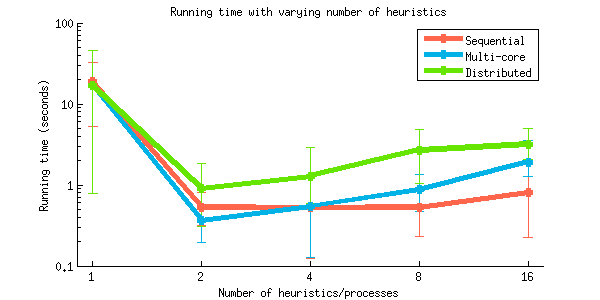
\includegraphics[width=3.2in]{graphs/figure1}
  \caption{Running time}
  \label{fig:singthread_runtime}
\end{subfigure}
\begin{subfigure}{3.2in}
  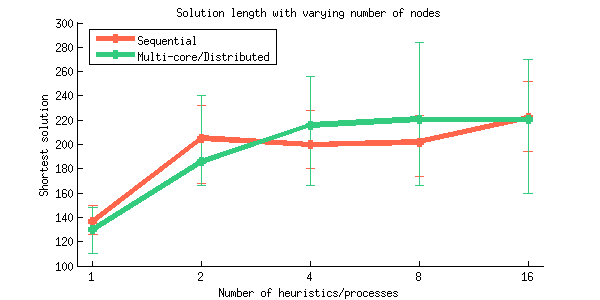
\includegraphics[width=3.2in]{graphs/figure2}
  \caption{Solution length}
  \label{fig:singthread_solnqual}
\end{subfigure}
\caption{Comparison with Runtime performance and solution quality as the number of different heuristics (cores) on a single machine increases.}
\label{fig:singthread}
\end{figure}

\begin{figure}
\centering
\begin{subfigure}{3.2in}
  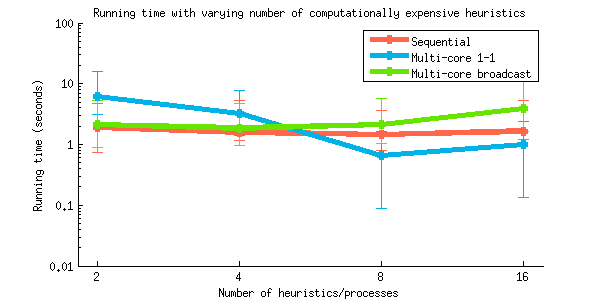
\includegraphics[width=3.2in]{graphs/figure3}
  \caption{Running time}
  \label{fig:numcores_runtime}
\end{subfigure}
\begin{subfigure}{3.2in}
  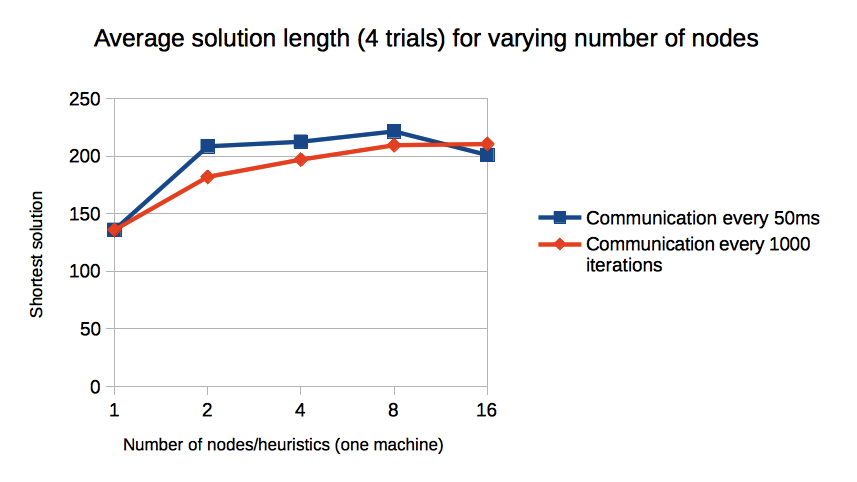
\includegraphics[width=3.2in]{graphs/numcores_solutionquality}
  \caption{Solution length}
  \label{fig:numcores_solnqual}
\end{subfigure}
\caption{Runtime performance and solution quality as the number of different heuristics (cores) on a single machine increases.}
\label{fig:numcores}
\end{figure}

\begin{figure}
\centering
\begin{subfigure}{3.2in}
  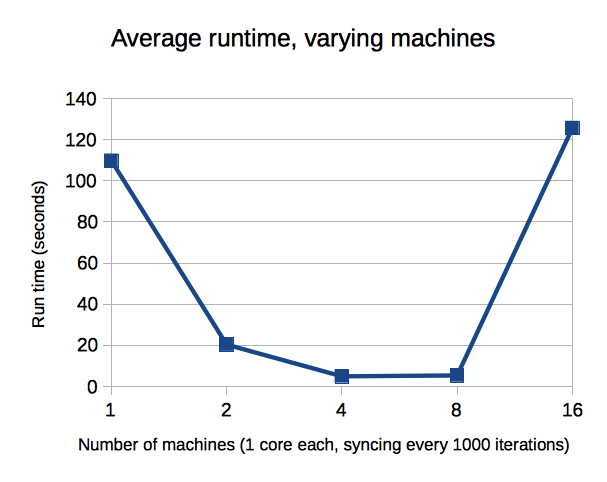
\includegraphics[width=3.2in]{graphs/nummachines_runningtime}
  \caption{Running time}
  \label{fig:nummachines_runtime}
\end{subfigure}
\begin{subfigure}{3.2in}
  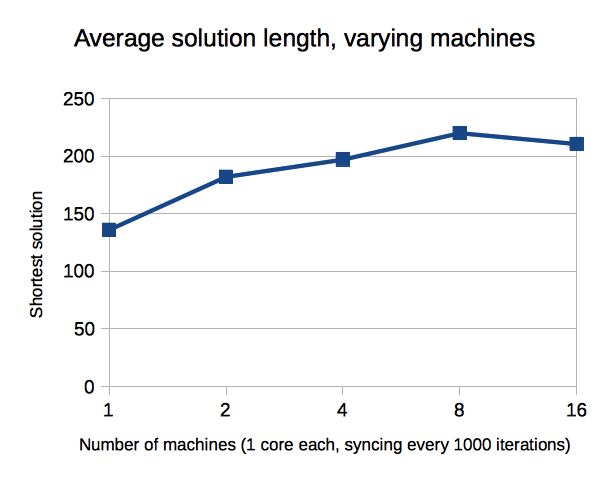
\includegraphics[width=3.2in]{graphs/nummachines_solutionquality}
  \caption{Solution length}
  \label{fig:nummachines_solnqual}
\end{subfigure}
\caption{Runtime performance and solution quality as the number of different machines (with one process each) increases from 1 to 16.}
\label{fig:nummachines}
\end{figure}

\begin{figure}
\centering
\begin{subfigure}{2.0in}
  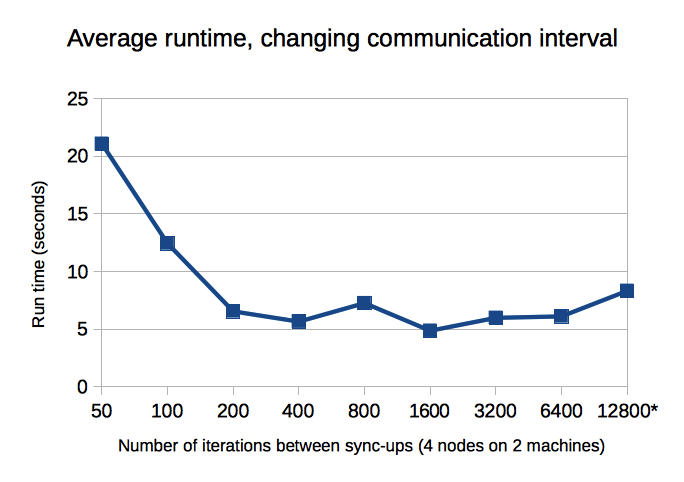
\includegraphics[width=2.0in]{graphs/commfreq_runningtime}
  \caption{Running time}
  \label{fig:commfreq_runtime}
\end{subfigure}
\begin{subfigure}{2.0in}
  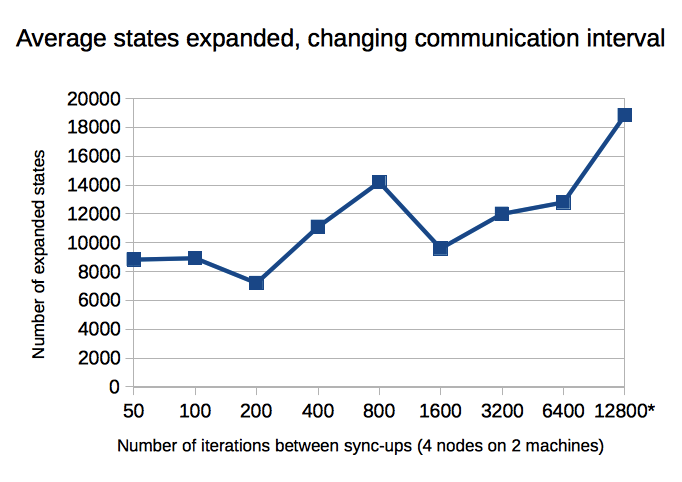
\includegraphics[width=2.0in]{graphs/commfreq_expansions}
  \caption{Number of state expansions}
  \label{fig:commfreq_expansions}
\end{subfigure}
\begin{subfigure}{2.0in}
  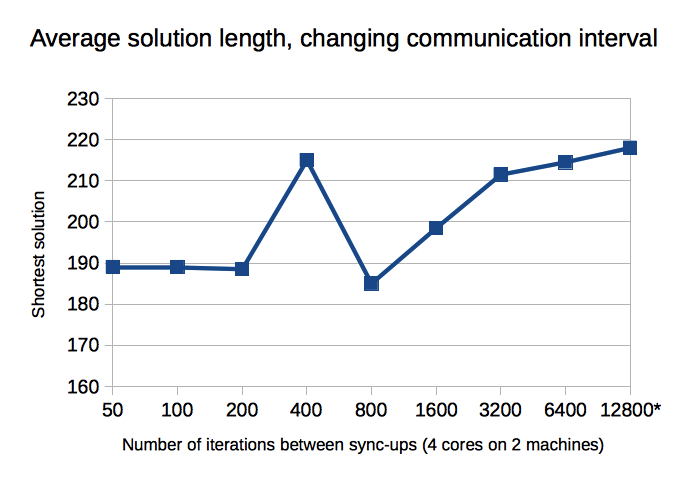
\includegraphics[width=2.0in]{graphs/commfreq_solutionquality}
  \caption{Solution length}
  \label{fig:nummachines_solnqual}
\end{subfigure}
\caption{Runtime performance, solution quality, and number of states expanded by the heuristic machines as the number of iterations between communication increases. *At the high end (12800 iterations between sync-ups), one of the four trials timed out (failed to find a solution within 5 minutes). The values in this graph are the average of the remaining three trials.}
\label{fig:commfreq}
\end{figure}



\begin{figure}
\centering
\begin{tabular}{ c | c | c | c }
    \hline
    \multicolumn{4}{c}{Single-threaded SMHA* implementation} \\ \hline    
    \# cores & time & \# expand & soln len \\ \hline
    1 & 1 & 2 & 3 \\ \hline
    2 & 4 & 5 & 6 \\ \hline
    4 & 7 & 8 & 9 \\ \hline
    % FILL USING AMPERSAND-SEPARATED VALUES WITH "\\ \hline" APPENDED AT THE END
    
     \multicolumn{4}{c}{Parallelized SMHA* (single machine, syncing every X iterations)} \\ \hline
    \# cores & time & \# expand & soln len \\ \hline
    % FILL USING AMPERSAND-SEPARATED VALUES WITH "\\ \hline" APPENDED AT THE END
    
     \multicolumn{4}{c}{Distributed SMHA* (one process per machine, syncing every X iterations)} \\ \hline
    \# machines & time & \# expand & soln len \\ \hline
    % FILL USING AMPERSAND-SEPARATED VALUES WITH "\\ \hline" APPENDED AT THE END
    
     \multicolumn{4}{c}{Distributed SMHA* with varying frequency of sync-ups} \\ \hline
     \multicolumn{4}{c}{(4 processes across 2 machines)} \\ \hline
    \# iterations & time & \# expand & soln len \\ \hline
    % FILL USING AMPERSAND-SEPARATED VALUES WITH "\\ \hline" APPENDED AT THE END

    \hline
\end{tabular}
\caption{Data from our trials}
\label{fig:datatable}
\end{figure}



\section{Conclusions}

% TODO: Fill me in!



% TODO: Should we have some kind of discussion on whether the parallelized version of SMHA* keeps the w1*w2 optimality guarantees that the single-threaded version does?? Also, maybe part of this, but the longer we go without doing a table update sync-up, the more the algorithm resembles IMHA*. It might be good to point this out somewhere, maybe in the Results/Discussion section




%\section{Final Paper Outline}

%\subsection{Introduction}
%\subsection{Related Work}
%\subsection{System Description}
%\subsection{Evaluation}
%\subsection{Conclusions and Future Work}

\bibliographystyle{ieeetr}
\bibliography{sources}


\end{document}